\chapter{Attack Model}\label{ch:attack}

In this chapter, we will extensively present the threat model of BREACH. We will
explain the conditions that should be met so as to launch the attack and
describe our code implementation for that case. Also, we will investigate the
types of vulnerabilities in web applications that can be exploited with this
attack, as well as introduce alternative secrets, that have not been taken into
consideration before.

\section{Mode of Operation}\label{sec:mo}

\subsection{Description}

The first step of the attack is for the attacker to gain control of the victim's
network, specifically being aple to view the victim's encrypted traffic. This
can be accomplished using the Man-in-the-Middle techniques described in Section
\ref{sec:mitm}.

After that the BREACH JavaScript that issues the requests needs to be executed
from the victim's browser. The first way to do this is to persuade the victim to
visit a website where the js runs, usually with social engineering methods, such
as phishing or spam email. Another way would be for the attacker to inject the
js code in a request made to a regular HTTP website. The following figure
depicts this methodology, which is based on the fact that regular HTTP traffic
is not encrypted and also does not ensure data integrity.

\begin{figure}[H] \caption{JavaScript injection.} \centering
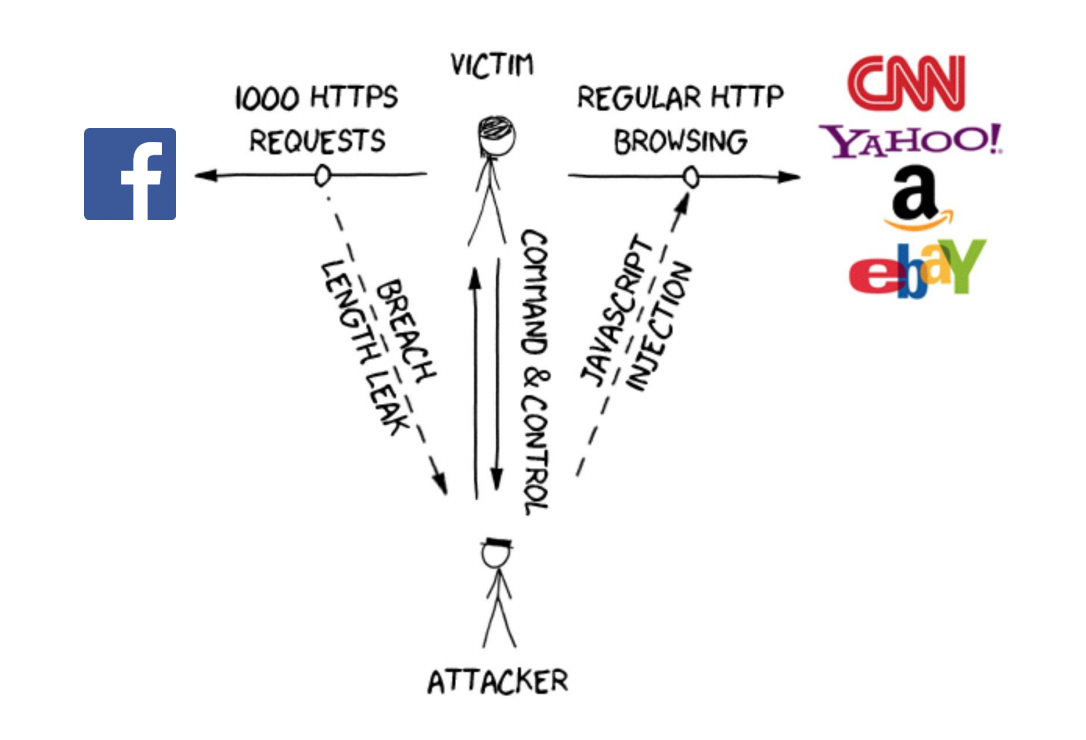
\includegraphics[width=0.6\textwidth]{diagrams/breach_mitm.png}\end{figure}

The script issues multiple requests to the target endpoint, which are sniffed by
the attacker. As described in Section \ref{sec:sameorigin} the attacker cannot
read the plaintext response, however the length of both the request and the
response is visible on the network.

Each request contains some data, that is reflected in the response. Since the
victim is logged in the target endpoint website, the response body will also
contain the secrets. If the conditions defined in Sections \ref{subsec:lz77} are
met, the secret and the reflected attacker input will be compressed and
encrypted.

By issuing a large amount of requests for different inputs, the attacker can
analyze the response lengths and extract information about the plaintext
secrets, as described above.

\subsection{Implementation}

For the implementation of the BREACH JavaScript, we assume the user has provided
the alphabet that the secret character we want to exfiltrate belongs to, as well
as the known prefix needed to bootstrap the attack.
